%%
%% The official i6 slide template _demo_
%% created by Philippe Dreuw and Thomas Deselaers, 2005
%%
%% $Id: slides.tex,v 1.48 2007-11-14 17:13:01 dreuw Exp $
%%
%% Possible options for:
%%  - language       : 'english' (default), 'german'
%%  - page numbering : 'nonumber', 'lastpage' to enable automatic page n/m numbering, 
%%                     'userlastpage' to enable a user defined page n/m numbering using \LastPage command,  
%%                      or leave empty for normal page numbering (default)
%%  - itemize        : 'triangle' or leave empty for bullets (default)
%%  - page titles    : 'allowpagebreaks' to enable titles with automatic page breaks, 
%%                     'nopagebreaks' to disable (default)
%%  - page layout    : 'vertical' to enable vertical centering on each slide using \vfill ... \vfill (default)
%%  - encoding       : 'utf-8' to enable utf encoding instead of latin1 (default)
%%  - tools          : 'blackslide' to insert a black slide which is linked with every slide title, e.g. to write a proof on the blackboard
%%
\documentclass[11pt, a4paper, landscape]{article}
\usepackage{NeyDreuwSlides_Nov07}

\usepackage{amsthm}
\newtheorem{definition}{Definition}
\newtheorem{theorem}{Theorem}[section]
\usepackage{algorithm}
\usepackage{algpseudocode}
\renewcommand{\algorithmicrequire}{\textbf{Input:}}
\renewcommand{\algorithmicensure}{\textbf{Output:}}

%%%%%%%%%%%%%%%%%%%%%%%%%%%%%%%%%%%%%%%%%%%%%%%%%%%%%%%%%%%%%%%%%%%%%%%%%%%%%%%%
%% flyspell can read the local ispelldict variable to automatically change the dictionary, 
%% e.g. german-new8, american, english, british, ...
%% 
%% Local IspellDict: american
%% 


%%%%%%%%%%%%%%%%%%%%%%%%%%%%%%%%%%%%%%%%%%%%%%%%%%%%%%%%%%%%%%%%%%%%%%%%%%%%%%%%
% custom packages
\usepackage{fancyvrb} %%% fancy verbatim to enable coloring within verbatim environments

%\usepackage{pst-node} 

%%%%%%%%%%%%%%%%%%%%%%%%%%%%%%%%%%%%%%%%%%%%%%%%%%%%%%%%%%%%%%%%%%%%%%%%%%%%%%%%
% Some example hacks work only in combination with the 'pdflatex -shell-escape'
% mode. Try 'make hacks'


%%%%%%%%%%%%%%%%%%%%%%%%%%%%%%%%%%%%%%%%%%%%%%%%%%%%%%%%%%%%%%%%%%%%%%%%%%%%%%%%
\renewcommand*{\title}{Graph-Based Image Segmentation}        % main title of the work (used for \TitlePage)
\renewcommand*{\titleshort}{Graph-Based Segmentation}         % short title (used for \lfoot)
\renewcommand*{\occasion}{Seminar Medical Image Processing -- MedBV13}		% (used for \TitlePage)
\renewcommand*{\occasionshort}{MedBV13}               % short occasion title (used for \rfoot)
%\renewcommand*{\date}{11. April 2005}                                        % default is \today (used for \TitlePage and \rfoot)
\renewcommand*{\author}{Phan-Anh Nguyen, Christian Oberdoefer}         % all the authors of the work, can be long (used for \TitlePage)
\renewcommand*{\authorshort}{Phan-Anh et al.:\xspace}                            % all the authors of the work, should be short (used for \lfoot)
\renewcommand*{\email}{\url{anh.nguyen@rwth-aachen.de, oberdoefer@i6.informatik.rwth-aachen.de}}  % all email address(es) of the authors (used for \TitlePage)
\renewcommand*{\mainauthor}{Phan-Anh Nguyen}                                   % the author(s) who presented the work (used for \TitlePage)
\renewcommand*{\mainauthoremail}{\url{anh.nguyen@rwth-aachen.de}}    % presenter mail address(es) (used for \FinalPage)
\renewcommand*{\www}{http://www-i6.informatik.rwth-aachen.de/}                % web address (used for \TitlePage _and_ \FinalPage)
\newcommand*{\keywords}{Graph Cut, Segmentation}                               % keywords, can be used for PDF summary

% will be set into the PDF document summary
\hypersetup{
  pdftitle={\title}, 
  pdfsubject={\occasion},  
  pdfauthor={\author}, 
  pdfkeywords={\keywords},
  % enable automatic page transitions: for endless loop edit in
  % acrobat reader -> preferences -> full screen -> after every X
  % seconds and after last page
  pdfpageduration = 2, 
%  pdfpagetransition = {Glitter /Di 315 /D 5}  
  pdfpagetransition = {Box /M /O /D 1},
}

%%%%%%%%%%%%%%%%%%%%%%%%%%%%%%%%%%%%%%%%%%%%%%%%%%%%%%%%%%%%%%%%%%%%%%%%%%%%%%%%
\listfiles
%%%%%%%%%%%%%%%%%%%%%%%%%%%%%%%%%%%%%%%%%%%%%%%%%%%%%%%%%%%%%%%%%%%%%%%%%%%%%%%%
\begin{document}

%%%%%%%%%%%%%%%%%%%%%%%%%%%%%%%%%%%%%%%%%%%%%%%%%%%%%%%%%%%%%%%%%%%%%%%%%%%%%%%%
\TitlePage

%%%%%%%%%%%%%%%%%%%%%%%%%%%%%%%%%%%%%%%%%%%%%%%%%%%%%%%%%%%%%%%%%%%%%%%%%%%%%%%%
\NewPage\headline{Outline}
%\small
\vfill
\begin{enumerate}
\item \hyperlink{sli:introduction}{Introduction and Motivation}
\item \hyperlink{sli:features}{Image Features}
%\begin{itemize}
%	\item \hyperlink{sli:surf}{Speeded Up Robust Features}
%	\item \hyperlink{sli:gPb}{Globalized Probability of Boundary}
%\end{itemize}
\item \hyperlink{sli:supervised}{Segmentation with Supervised Training}
%\begin{itemize}
%	\item \hyperlink{sli:svm}{Support Vector Machine for Region Ranking}
%	\item \hyperlink{sli:logistic}{Logistic Regression}
%	\item \hyperlink{sli:ssm}{Statistical Shape Model}
%\end{itemize}
\item \hyperlink{sli:construction}{Graph Construction}
\begin{itemize}
	\item \hyperlink{sli:region_graph}{Region Graph}
	\item \hyperlink{sli:contour_graph}{Contour Graph}
	\item \hyperlink{sli:mrf}{Markov Random Field}
\end{itemize}
\item \hyperlink{sli:algorithms}{Graph Cut Algorithms}
%\begin{itemize}
%	\item \hyperlink{sli:PCST}{Prize-Collecting Steiner Tree}
%	\begin{itemize}
%		\item \hyperlink{sli:branch_and_cut}{Branch-and-Cut Algorithm}
%	\end{itemize}
%	\item \hyperlink{sli:contour_cut}{Contour Cut}
%	\begin{itemize}
%		\item \hyperlink{sli:circulation}{Graph Circulations}
%		\item \hyperlink{sli:cost}{The Cost Function}
%		\item \hyperlink{sli:solution}{Computational Solution}
%	\end{itemize}
%	\item \hyperlink{sli:graph_cut}{Graph-Cut}
%	\begin{itemize}
%		\item \hyperlink{sli:min_cut}{Min-Cut Algorithm}
%		\item \hyperlink{sli:multi_shape}{Multi-Shape Graph-Cuts}
%	\end{itemize}
%\end{itemize}
\item \hyperlink{sli:application}{Applications}
%\begin{itemize}
%	\item \hyperlink{sli:ERS}{Efficient Region Search for Object Detection}
%	\item \hyperlink{sli:contour_detector}{Salient Contour Detection}
%	\item \hyperlink{sli:lung_segmentation}{Multi-Shape Graph-Cut for Lung Segmentation}
%\end{itemize}
\item \hyperlink{sli:conclusion}{Conclusion}
\end{enumerate}
\vfill
%\centerline{\footnotesize PS: the outline should not have more than 5-7 items
%  without any subitems}
%\normalsize
%\vfill


%%%%%%%%%%%%%%%%%%%%%%%%%%%%%%%%%%%%%%%%%%%%%%%%%%%%%%%%%%%%%%%%%%%%%%%%%%%%%%%%
\NewPage\headline{Literature} 
\vfill 
\begin{itemize}
\item S. Vijayanarasimhan and K. Grauman. \alert{Efficient region search for object detection.} Computer Vision and Pattern Recognition (CVPR), 2011 IEEE Conference, pages 1401--1408, June 2011.
\item R. Kennedy, J. Gallier, and Jianbo Shi. \alert{Contour cut: Identifying salient contours in images
by solving a hermitian eigenvalue problem.} Computer Vision and Pattern Recognition (CVPR), 2011 IEEE Conference, pages 2065--2072, June 2011.
\item Nakagomi, K. and Shimizu, A. and Kobatake, H. and Yakami, M. and Fujimoto, K. and Togashi, K. \alert{Multi-shape graph-cuts and its application to lung segmentation from a chest CT volume.}
\end{itemize}
\vfill


%%%%%%%%%%%%%%%%%%%%%%%%%%%%%%%%%%%%%%%%%%%%%%%%%%%%%%%%%%%%%%%%%%%%%%%%%%%%%%%%
\NewPage\headline{Introduction and Motivation} 
\hypertarget{sli:introduction}
\vfill
\begin{itemize}
\item Purposes of segmentation
\begin{itemize}
	\item Computer-aided diagnoses
	\item Object detection and segmentation for autonomous systems
	\item Shape alignments
\end{itemize}
\item Current problems
\begin{itemize}
	\item deformable shapes
	\item time constraint
	\item no clear boundaries
\end{itemize}
\item Advantages of Graph Representation
%\begin{itemize}
%	\item Flexible expression of constraints 
%	\item Powerful graph algorithms exist\\
%	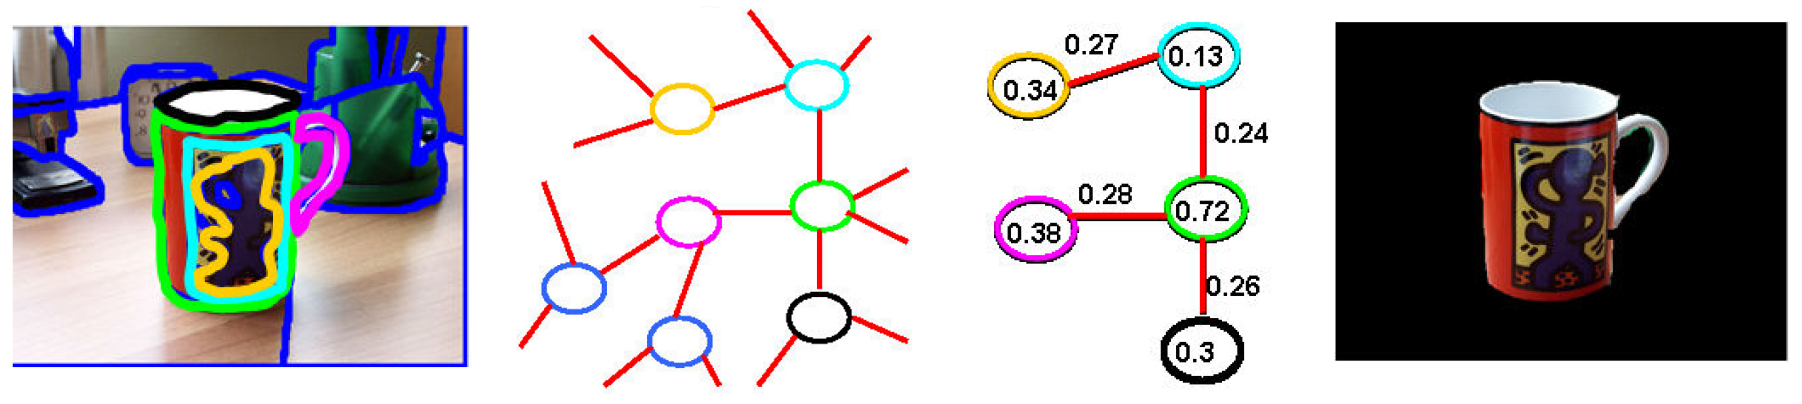
\includegraphics[width=.6\linewidth]{region_graph_intro}
%\end{itemize}
\begin{table}
  \centering
  \begin{tabular}{@{} M{.4\linewidth} M{.6\linewidth} @{}}
  	\begin{itemize}
  		\item Flexible expression of constraints 
  		\item Powerful graph algorithms exist
    \end{itemize}
      &
    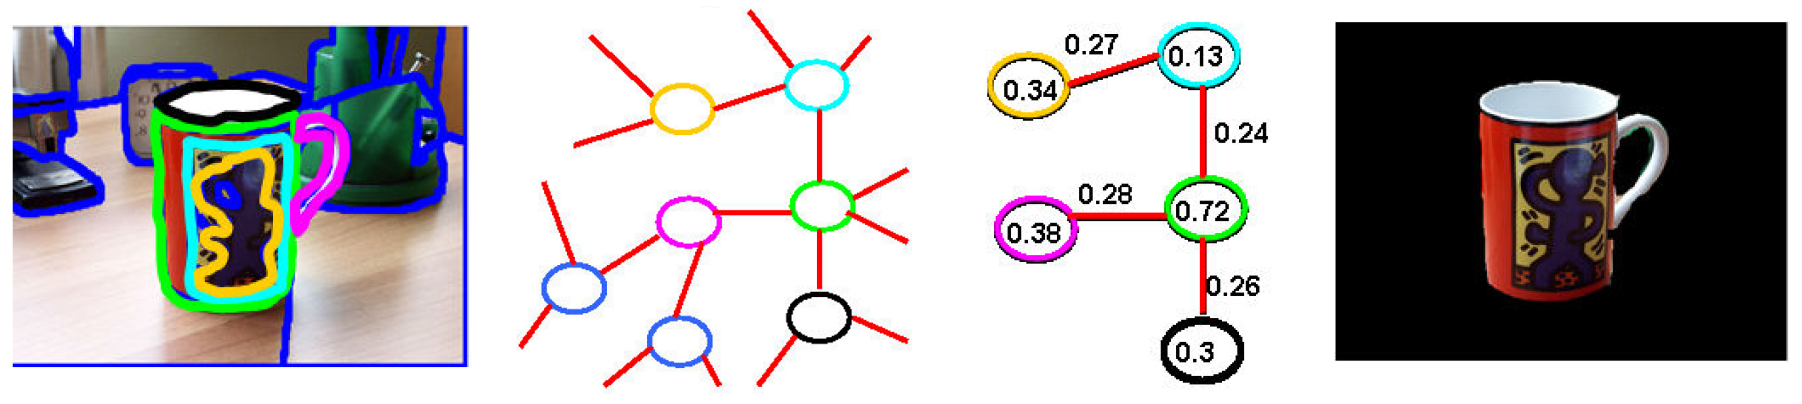
\includegraphics[width=.9\linewidth]{region_graph_intro}
  \end{tabular}
\end{table}

\end{itemize}
\vfill



%%%%%%%%%%%%%%%%%%%%%%%%%%%%%%%%%%%%%%%%%%%%%%%%%%%%%%%%%%%%%%%%%%%%%%%%%%%%%%%%
\NewPage\headline{Image Features: Speeded Up Robust Features}
\hypertarget{sli:style}
\vfill
\begin{itemize}
\item Detect interest points: $det(Hessian(I)) = I_{xx}I_{yy} - I^2_{xy}$
\item Orientation assignment (rotation invariant): select the dominant direction of Haar wavelet response vectors $(d_x, d_y)$.
\item SURF is computed within a window of size $20s$.
\item Further split the window into $4 \times 4$ sub-windows.
\item[]
  \begin{figure}
    \centering
    \begin{tabularx}{600pt}{Z Z Z}
      
\includegraphics[height=2.0cm]{haar_wavelet}%
      \caption{Haar wavelet filters}%
      &
      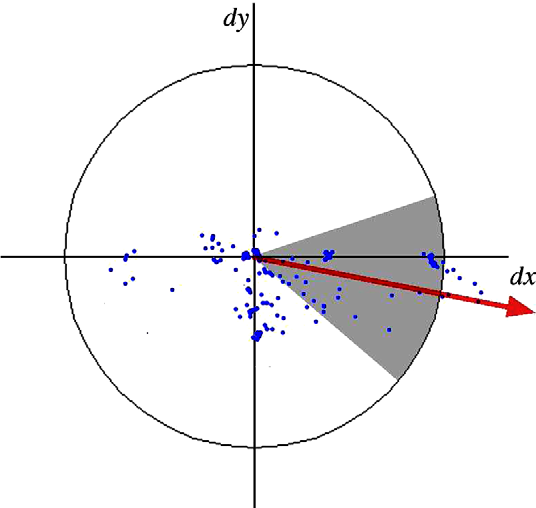
\includegraphics[height=5.5cm]{orientation_window}%
      \caption{sum $(d_x, d_y)$ over a window size $\frac{\pi}{3}$}%
      &
      \includegraphics[height=5.5cm]{feature_neighborhood}%
      \caption{windows defining neighborhood}%
    \end{tabularx}
  \end{figure}
\end{itemize}
\vfill


%%%%%%%%%%%%%%%%%%%%%%%%%%%%%%%%%%%%%%%%%%%%%%%%%%%%%%%%%%%%%%%%%%%%%%%%%%%%%%%%
\NewPage\headline{Image Features: Speeded Up Robust Features}
\vfill
\begin{itemize}
\item 4D descriptor vector $v = (\sum d_x, \sum d_y, \sum \lvert d_x \rvert, \sum \lvert d_y \rvert)$ for each sub-window $\Rightarrow$ 64D SURF descriptor.
\item Normalize to make it invariant to contrast (a scale factor).
%\item[]
\end{itemize}
  \begin{figure}
    \centering
    \begin{tabularx}{600pt}{Z Z}
      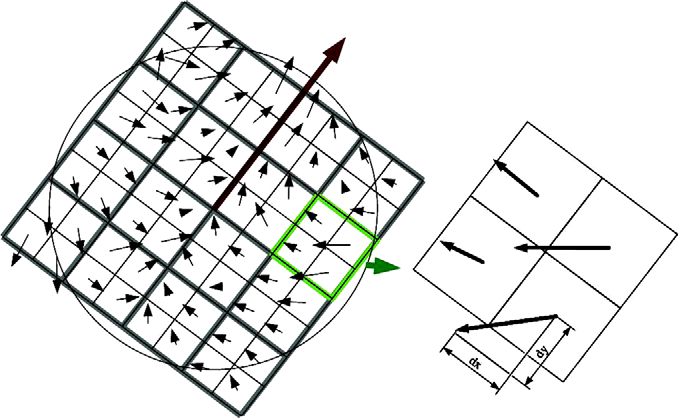
\includegraphics[width=0.4\textwidth]{surf}%
      \caption{Wavelet responses extracted from neighborhood}%
      &
      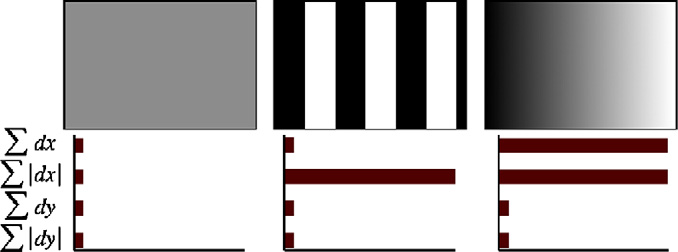
\includegraphics[width=0.4\textwidth]{surf_vector}%
      \caption{The descriptor entries represent the underlying intensity pattern.}%
    \end{tabularx}
  \end{figure}
\vfill


%%%%%%%%%%%%%%%%%%%%%%%%%%%%%%%%%%%%%%%%%%%%%%%%%%%%%%%%%%%%%%%%%%%%%%%%%%%%%%%%
\NewPage\headline{Gradient-based Features}
\small
\vfill
\begin{itemize}
\item Draw a circle with radius $r$, divide it along the diameter at orientation $\theta$.
\item Build histograms of brightness, color and texture for each disc half.
\item Compares histograms of the two disc halves: $G(x, y, \theta, r) = \chi ^ 2 (g, h) = \frac{1}{2} \sum_i \frac{(g_i - h_i)^2}{(g_i + h_i)}$
\item Use logistic regression trained on human segmentation dataset to get the result $Pb_{\sigma}(x, y, \theta)$.
\end{itemize}
\begin{figure}
	\centering
	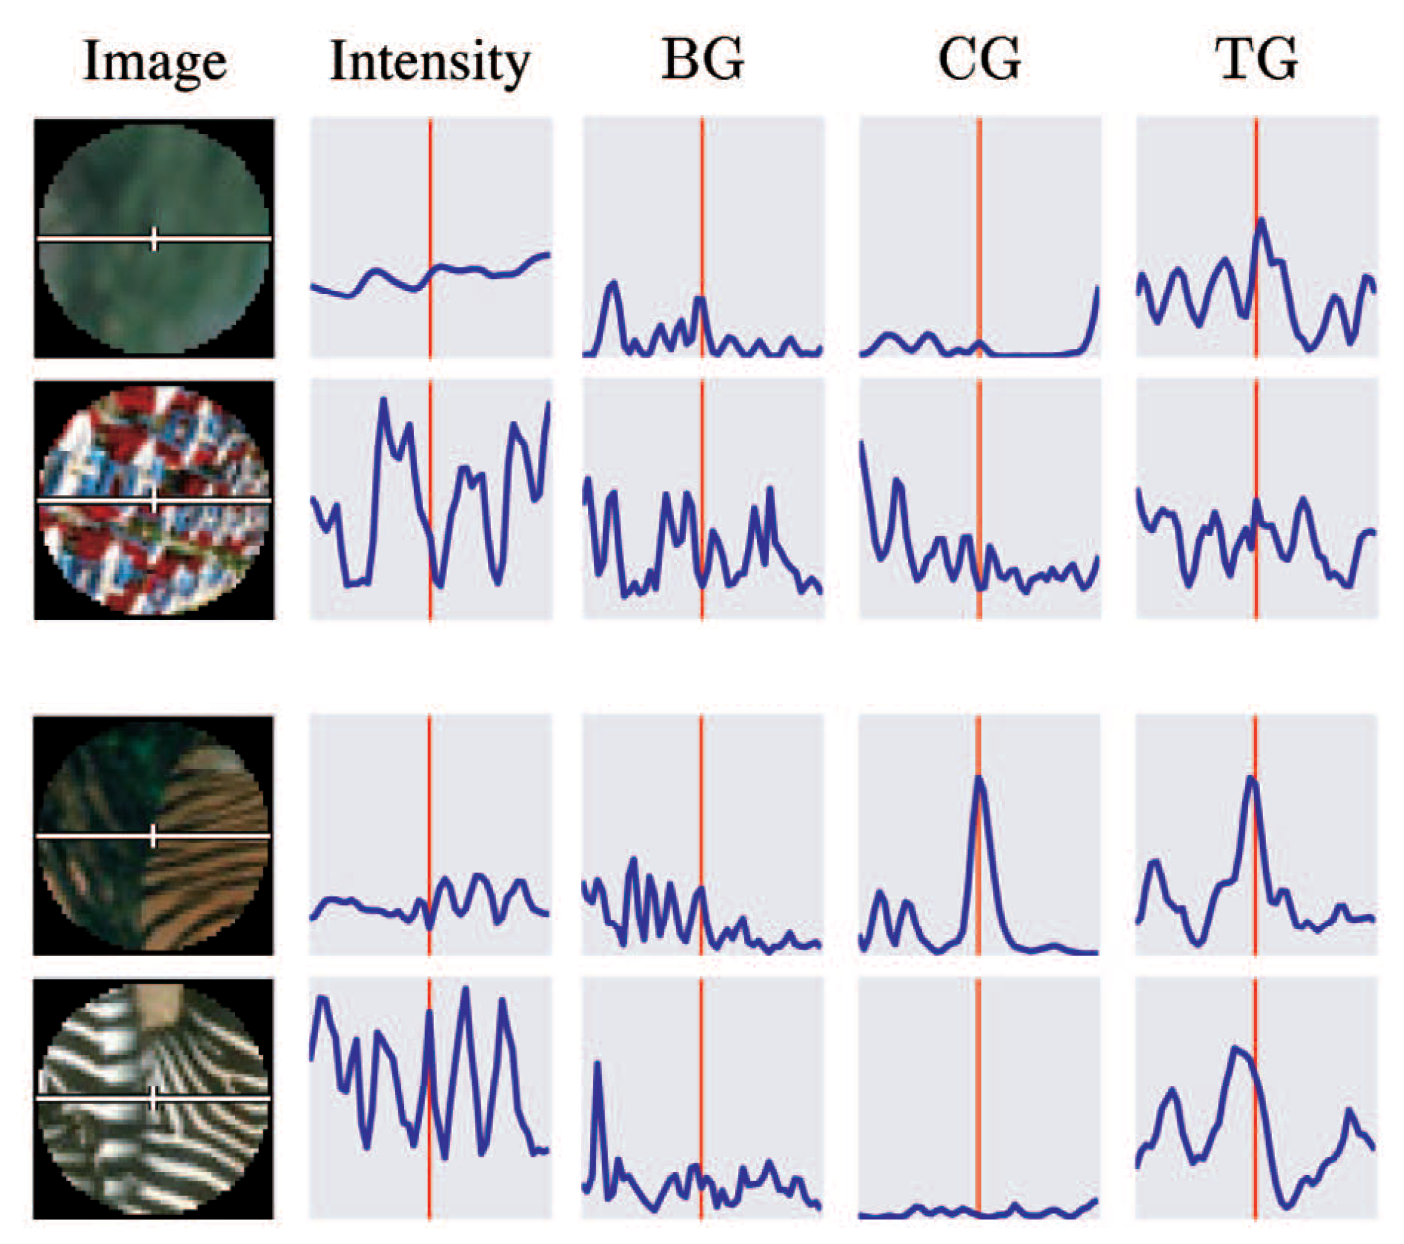
\includegraphics[width=0.45\textwidth]{gradient_features}
\end{figure}
\vfill


%%%%%%%%%%%%%%%%%%%%%%%%%%%%%%%%%%%%%%%%%%%%%%%%%%%%%%%%%%%%%%%%%%%%%%%%%%%%%%%%
\NewPage\headline{Globalized Probability of Boundary}
\small
\vfill
\begin{itemize}
\item Brightness, color and texture gradients in 3 different scales: $mPb(x, y, \theta) = \sum\limits_{i = 1}^{9} G_i(x, y, \theta)$.
\item Define affinity matrix $W$ using intervening contour cue $mPb$. Solve the generalized eigenvectors problem: $(D - W)v = \lambda D v$, $D_{ii} = \sum_j W_{ij}$.
\item Edges from generalized eigenvectors $v_j$: $sPb(x, y, \theta) = \sum\limits_{j = 1}^{k} \frac{1}{\sqrt{\lambda_j}} sPb_{v_j} (x, y, \theta)$.
\item Globalized probability of boundary: $gPb(x, y, \theta) = \sum\limits_{i = 1}^{9} \beta_iG_i(x, y, \theta) + \gamma sPb(x, y, \theta)$.
\end{itemize}
%  \begin{figure}
%    \centering
%    \begin{tabularx}{600pt}{Z Z}
%      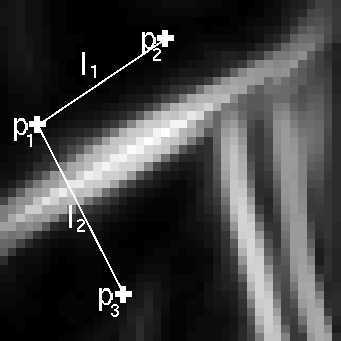
\includegraphics[width=0.15\textwidth]{intervening_contour2}%
%      \caption{Intervening contour}%
%      &
%      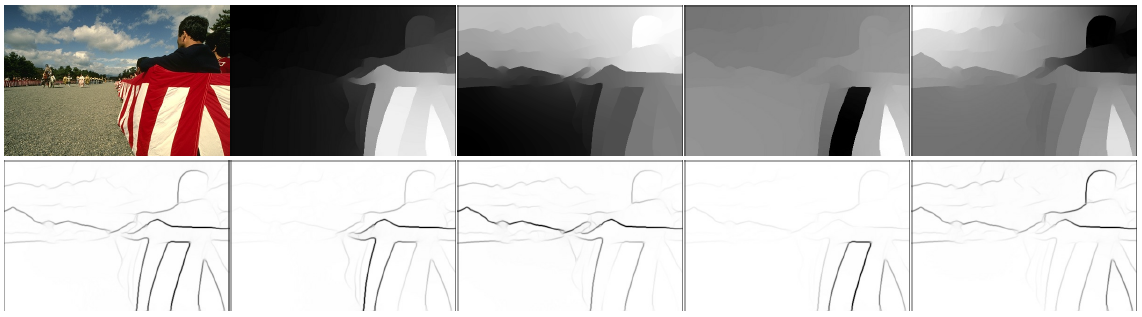
\includegraphics[width=0.55\textwidth]{sPb}%
%      \caption{Eigenvectors and their edges}%
%    \end{tabularx}
%  \end{figure}
\begin{table}
  \centering
  \begin{tabular}{@{} M{.3\linewidth} M{.7\linewidth} @{}}
      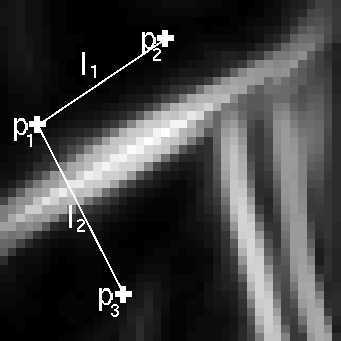
\includegraphics[width=0.15\textwidth]{intervening_contour2}%
      \caption{Intervening contour}%
      &
      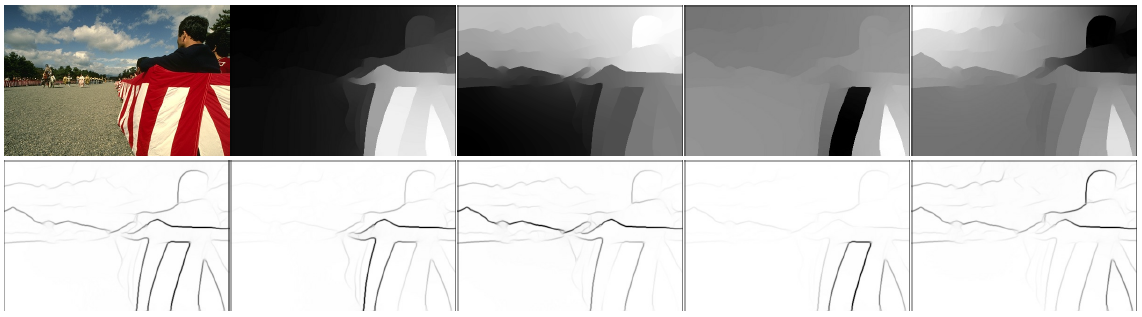
\includegraphics[width=0.65\textwidth]{sPb}%
      \caption{Eigenvectors and their edges}%
  \end{tabular}
\end{table}
\vfill


%%%%%%%%%%%%%%%%%%%%%%%%%%%%%%%%%%%%%%%%%%%%%%%%%%%%%%%%%%%%%%%%%%%%%%%%%%%%%%%%
\NewPage\headline{Support Vector Machine}
\vfill
\begin{itemize}
\item Given training data $\left\lbrace (h_i, t_i) \right\rbrace _{i = 1} ^S$, find a classifier $f(h) = w^Th + b$ that maximizes the margin.
\item Equivalent to find a hyperplane satisfying: $\arg\min\limits_{w, b} \frac{1}{2} \|w\| ^2, \qquad t_i(w^Th_i + b) \geq 1 \forall i$.
\item The solution for $w$ is a linear combination of training examples: $w = \sum\limits_{i = 1}^{S} a_it_ih_i = \sum\limits_{i = 1}^{S} \alpha_ih_i$.
\end{itemize}
\begin{figure}
	\centering
	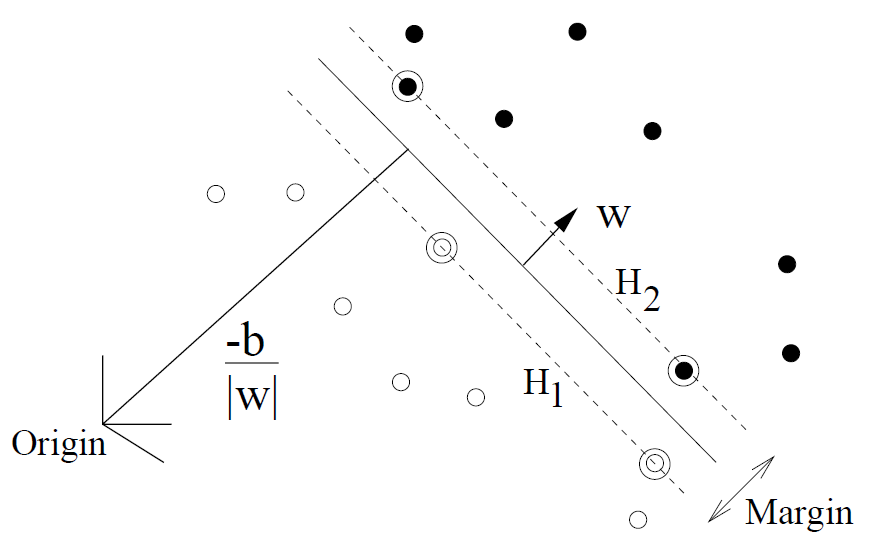
\includegraphics[width=0.5\textwidth]{svm}
\end{figure}
\vfill


%%%%%%%%%%%%%%%%%%%%%%%%%%%%%%%%%%%%%%%%%%%%%%%%%%%%%%%%%%%%%%%%%%%%%%%%%%%%%%%%
\NewPage\headline{SVM for Region Ranking}
\vfill
\begin{figure}
	\centering
	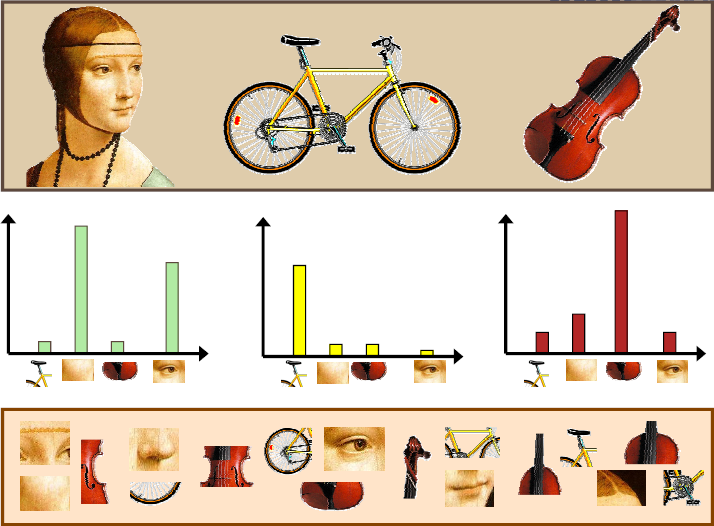
\includegraphics[width=0.45\textwidth]{bag_of_features}
	\caption{Bag of visual words}
\end{figure}
\begin{itemize}
\item Region $R = \left\lbrace (x_i, v_i) \right\rbrace _{i = 1} ^N$, its ranking score $f(R) = b + (\sum_i\alpha_ih(R_i)) \cdot h(R)$.
\item Associate each $j$-th word with a weight $w_j = \sum_i\alpha_ih_j(R_i)$.
\item $f(R) = b + \sum\limits_{j = 1}^{K} w_jh_j(R) = b + \sum\limits_{i = 1}^{N} w_{d_i}$, 
\item $d_i \in \left[ 1, K \right] $ the index of the visual word that feature $v_i$ maps to.
\end{itemize}
\vfill



%%%%%%%%%%%%%%%%%%%%%%%%%%%%%%%%%%%%%%%%%%%%%%%%%%%%%%%%%%%%%%%%%%%%%%%%%%%%%%%%
\NewPage\headline{Region Graph}
\vfill
\begin{itemize}
\item Watershed to define regions from gPb contours
\item Vertex weights: SVM on SURF and Shape descriptors. Edge weights: intervening contour strengths
\item $f^{\prime}(R) = \sum\limits_{i = 1}^{N}w^v_{d_i} - \sum\limits_{j = 1}^{M} w^e_{s_j}$, $s_j \in \left[ 1, L \right] $ is the bin index of the contour strength histogram for the $j^{th}$ contour.
\end{itemize}
\begin{figure}
	\centering
	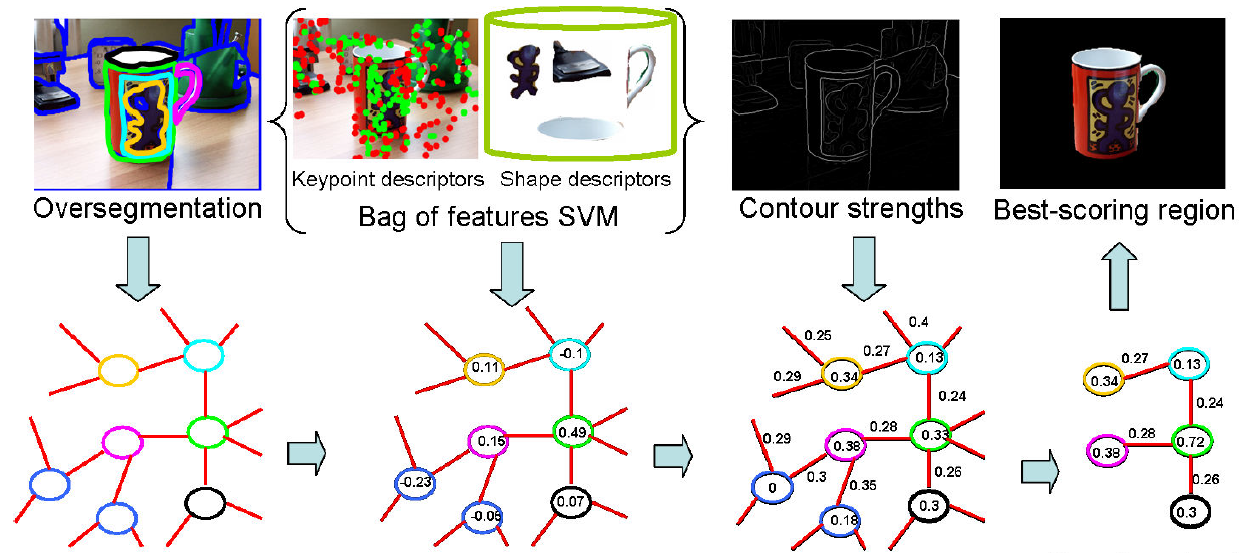
\includegraphics[width=0.8\textwidth]{region_graph}
\end{figure}
\vfill


%%%%%%%%%%%%%%%%%%%%%%%%%%%%%%%%%%%%%%%%%%%%%%%%%%%%%%%%%%%%%%%%%%%%%%%%%%%%%%%%
\NewPage\headline{Prize-Collecting Steiner Tree Problem}
\vfill
\begin{definition}
PCST PROBLEM: Given a connected undirected vertex and edge weighted graph G = (V, E, c, p) with vertex profits $p: V \rightarrow \mathbb{R}^{\geq 0}$ and edge costs $c: E \rightarrow \mathbb{R}^{\geq 0}$, find a connected subgraph T = ($V_T \subseteq V, E_T \subseteq E$) of G that maximizes the profit:
\begin{equation}
P(T) = \sum\limits_{v \in V_T} p(v) - \sum\limits_{e \in E_T} c(e)
\end{equation}
\end{definition}
\begin{itemize}
\item Optimal solution: branch-and-cut algorithm
\item Efficient for hundreds of nodes
\end{itemize}
\vfill


%%%%%%%%%%%%%%%%%%%%%%%%%%%%%%%%%%%%%%%%%%%%%%%%%%%%%%%%%%%%%%%%%%%%%%%%%%%%%%%%
\NewPage\headline{Contour Graph}
\vfill
\begin{itemize}
\item Threshold edge detector output to get edge segments: edgels.
\item Duplicate each edgel into $i$ and $\bar{i}$ with opposite directions $\theta, \theta + \pi$.
\item Connect pairs of edgels within some distance $r_e$: $E = \left\lbrace (i, j) : \| (x_i, y_i) - (x_j, y_j) \| \leq r_e \right\rbrace $.
\item Weights measure directed collinearity: $W_{ij} = e^{-(1 - cos(\mid \phi_i \mid + \mid \phi_j \mid))/\sigma^2}\ \mathrm{if}\ i \rightarrow j$.
\item Curve $\Rightarrow$ two chains $\Rightarrow$ convert into a cycle by adding an edge between terminal points.
\end{itemize}
\begin{figure}
	\centering
	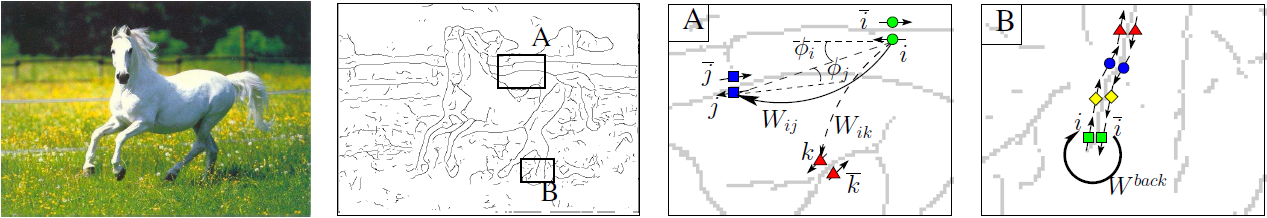
\includegraphics[width=0.95\textwidth]{contour_graph}
\end{figure}
\vfill


%%%%%%%%%%%%%%%%%%%%%%%%%%%%%%%%%%%%%%%%%%%%%%%%%%%%%%%%%%%%%%%%%%%%%%%%%%%%%%%%
\NewPage\headline{Circular Embedding}
\vfill
\begin{itemize}
\item A contour $(C, O)$ consists of a set of vertices $C$ and an ordering function $O: C \rightarrow \left\lbrace 1, ..., \lvert C \rvert \right\rbrace $
\item Each node of the contour is mapped to a point on a complex circle, all other points are mapped to the origin.
\item $x_j = r_j\exp(i\theta_j)$, $r_j = 1$ if $j \in C$ and 0 otherwise,
\item $\theta_j = O(j)\delta$, where $\delta = \frac{2\pi}{\lvert C \rvert}$ is a phase step.
\end{itemize}
\begin{figure}
	\centering
	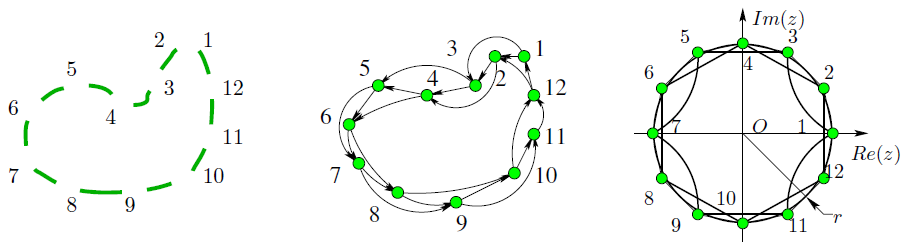
\includegraphics[width=0.7\textwidth]{circular_embedding}
\end{figure}
\vfill


%%%%%%%%%%%%%%%%%%%%%%%%%%%%%%%%%%%%%%%%%%%%%%%%%%%%%%%%%%%%%%%%%%%%%%%%%%%%%%%%
\NewPage\headline{Markov Random Field}
\vfill
\begin{itemize}
\item Nodes are random variables $\left\lbrace x_1, ..., x_n \right\rbrace $ corresponding to pixels.
\item Two types of edges: neighborhood relation, correlation between true state and observed data
\item A graph represents a joint distribution $p(x)$
\item Can be written as a product of potential functions $\psi_C(x_C)$ over the maximal cliques:
\item[]
	\begin{center}
		$p(x) = \frac{1}{Z} \prod\limits_{C}\psi_C(x_C)$
	\end{center}
\item Conveniently expressed as energy functions: $\psi_C(x_C) = \exp(-E(x_C))$.
\item Maximize $p(x)$ equals to minimize $E$.
\end{itemize}
\begin{table}
  \centering
  \begin{tabular}{@{} M{.5\linewidth} M{.5\linewidth} @{}}
      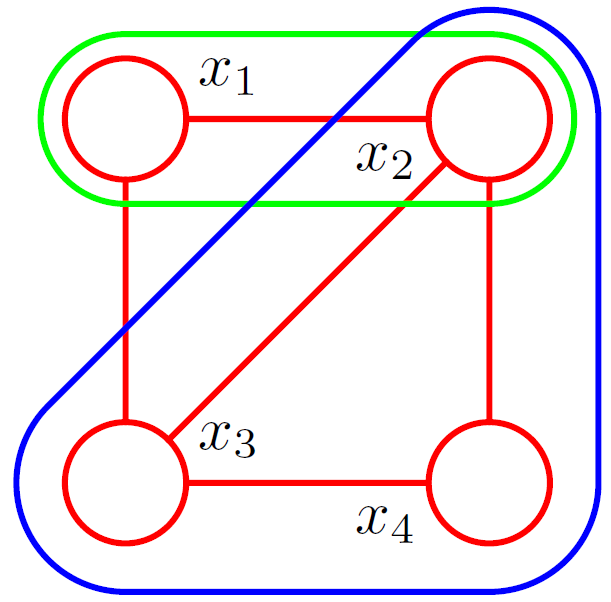
\includegraphics[width=0.2\textwidth]{clique}%
      \caption{Cliques}%
      &
      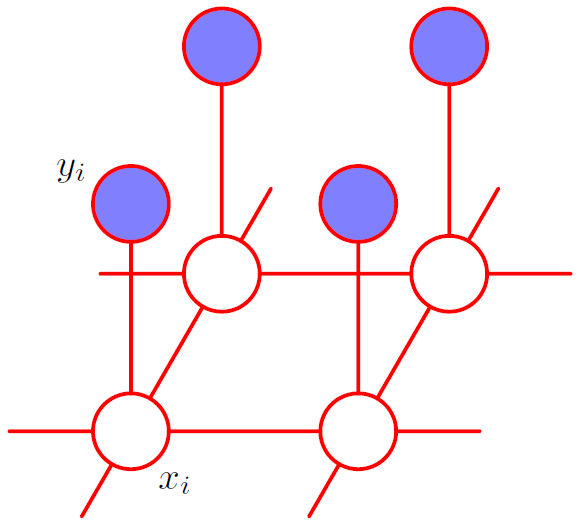
\includegraphics[width=0.2\textwidth]{mrf}%
      \caption{MRF}%
  \end{tabular}
\end{table}
\vfill


%%%%%%%%%%%%%%%%%%%%%%%%%%%%%%%%%%%%%%%%%%%%%%%%%%%%%%%%%%%%%%%%%%%%%%%%%%%%%%%%
\NewPage\headline{Shape Energy}
\vfill
\begin{itemize}
\item Given label set $L = \left\lbrace 1, ..., l \right\rbrace $, find labelling $A = (A_1, ..., A_{\lvert P \rvert})$ minimizing energy:
\begin{center}
$E(A) = \lambda \sum\limits_{p \in P} R_p(A_p) + \sum\limits_{(p, q) \in \mathcal{N}} (B_{p, q} + S_{p, q})\delta_{A_p \neq A_q}$,
\end{center}
\item[]
\begin{center}
$S_{p, q} = \min(\mathrm{sqrt}\left\lbrace [1 - \cos(\theta_{A_p})]/2 \right\rbrace, \mathrm{sqrt}\left\lbrace [1 - \cos(\theta_{A_q})]/2 \right\rbrace )$
\end{center}
\end{itemize}
\begin{figure}
	\centering
	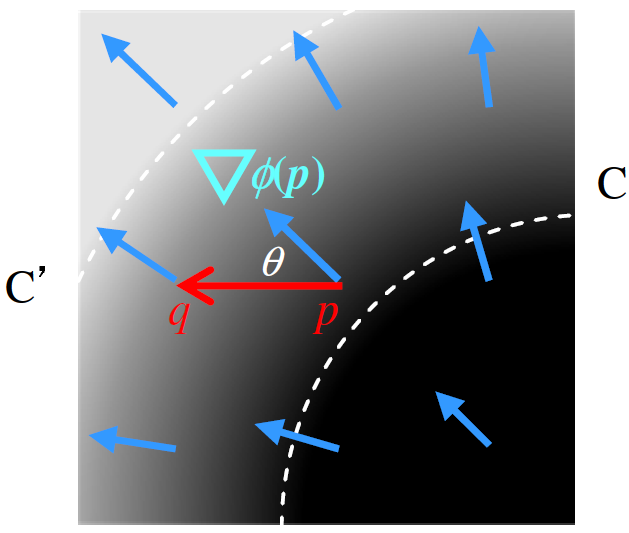
\includegraphics[width=0.4\textwidth]{shape_energy}
	\caption{True shape $C^{\prime}$ is similar to shape prior $C$}
\end{figure}
\vfill


%%%%%%%%%%%%%%%%%%%%%%%%%%%%%%%%%%%%%%%%%%%%%%%%%%%%%%%%%%%%%%%%%%%%%%%%%%%%%%%%
\NewPage\headline{Integer Linear Programing formulation of PCST}
\vfill
\begin{itemize}
\item The PCST can be formulated as an ILP problem with $n$ variables and $m$ constraints:
\item[]
\begin{center}
$\min \left\lbrace c^Tx : Ax \geq b, x \in \mathbb{Z}_+^n \right\rbrace $
\end{center}
\item $x \in \mathbb{Z}_+^n$ integer decision variables, $c \in \mathbb{Z}^n$ objective function vector and $A \in \mathbb{Z}^{m \times n}$ the matrix of constraint coefficients.
\item The LP-relaxation (CUT) is obtained by using real-value constraints $x \in \mathbb{R}_+^n$.
\item Its feasible region is the polyhedron:
\item[]
\begin{center}
$P = \left\lbrace x \in \mathbb{R}_+^n : Ax \geq b \right\rbrace $
\end{center}
\item The integral hull of the set of integer solutions, i.e., the polyhedron:
\item[]
\begin{center}
$P_I = \mbox{conv} \left\lbrace x \in \mathbb{Z}_+^n : Ax \geq b \right\rbrace $
\end{center}
%\item A cutting plane as a linear inequality that is valid for $P_I$ but not for $P$.
\begin{table}
  \centering
  \begin{tabular}{@{} M{.5\linewidth} M{.5\linewidth} @{}}
  \begin{itemize}
  	\item A cutting plane is a linear inequality that is valid for $P_I$ but not for $P$.
  \end{itemize}
      &
    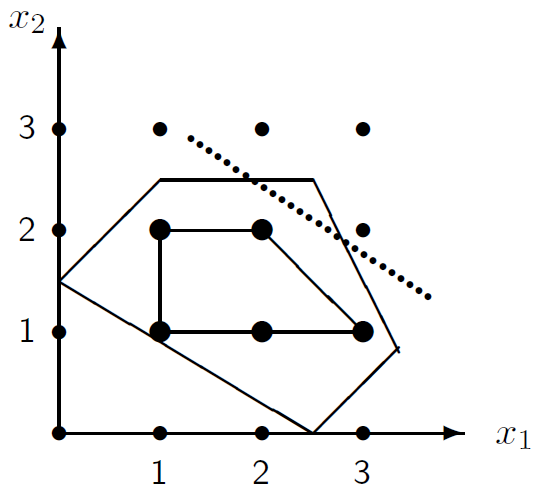
\includegraphics[width=0.25\textwidth]{cutting_plane}
  \end{tabular}
\end{table}
\end{itemize}
%\begin{figure}
%	\centering
%	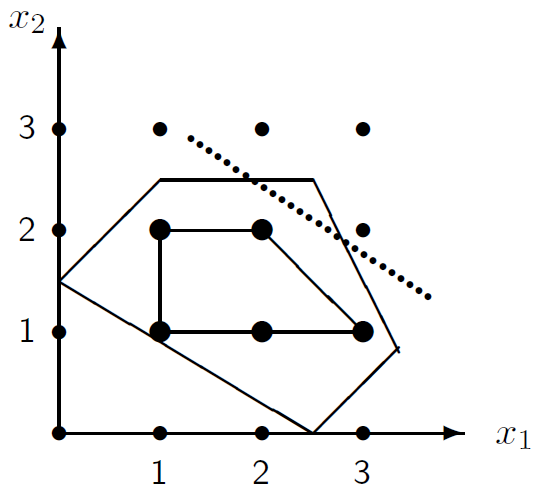
\includegraphics[width=0.2\textwidth]{cutting_plane}
%\end{figure}
\vfill



%%%%%%%%%%%%%%%%%%%%%%%%%%%%%%%%%%%%%%%%%%%%%%%%%%%%%%%%%%%%%%%%%%%%%%%%%%%%%%%%
\NewPage\headline{Branch-and-Cut Example}
\vfill
\begin{itemize}
\item The integer programming problem (Eg0):
%\item[]
\begin{table}
  \centering
  \begin{tabular}{l l}
  	$\min$ 		& $z = -6x_1 - 5x_2$\\
	subject to  & $3x_1 + x_2 \leq 11$\\
                & $-x_1 + 2x_2 \leq 5$\\
                & $x_1, x_2 \geq 0$, interger.
  \end{tabular}
\end{table}
\item Solve the linear programming relaxation.
\item Branch on $x_1$ to get two new problems:
\begin{itemize}
\item Add constraint $x_1 \geq 3$ to Eg0 to get Eg1 $\Rightarrow$ integral solution (3, 2), with value -28.
\item Add constraint $x_1 \leq 2$ to Eg0 to get Eg2 $\Rightarrow$ solution (2, 3.5), with value -29.5.
\end{itemize}
\item Add a cutting plane $2x_1 + x2 \leq 7$ to Eg2 to get Eg3 $\Rightarrow$ solution (1.8, 3.4), with value -27.8.
\item The solution of Eg3 is larger than the integral solution of Eg1 $\Rightarrow$ terminate.
\end{itemize}
\vfill


%%%%%%%%%%%%%%%%%%%%%%%%%%%%%%%%%%%%%%%%%%%%%%%%%%%%%%%%%%%%%%%%%%%%%%%%%%%%%%%%
\NewPage\headline{Branch-and-Cut Example}
\vfill
\begin{figure}
	\centering
	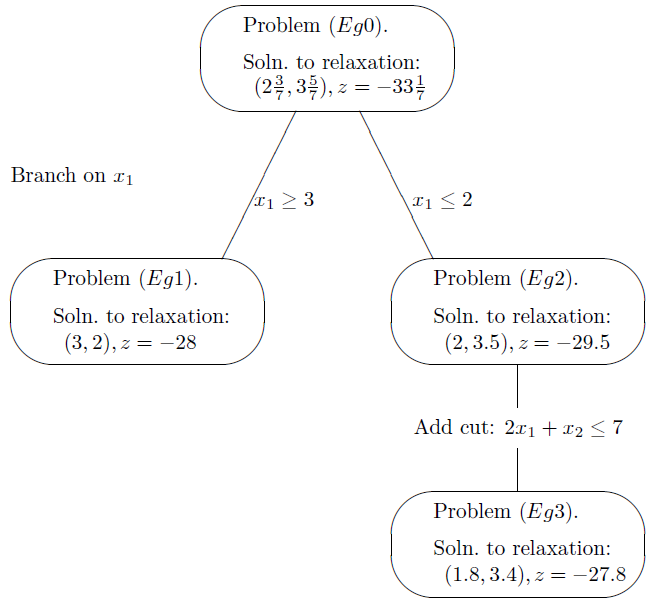
\includegraphics[width=0.55\textwidth]{branch_and_cut}
\end{figure}
\vfill


%%%%%%%%%%%%%%%%%%%%%%%%%%%%%%%%%%%%%%%%%%%%%%%%%%%%%%%%%%%%%%%%%%%%%%%%%%%%%%%%
\NewPage\headline{Contour Cut: Graph Circulations}
\small
\vfill
\begin{definition}
A matrix $F \in (\mathbb{R}^+ \cup \left\lbrace 0 \right\rbrace )^{\lvert V \rvert \times \lvert V \rvert}$ that assigns each directed edge to a non-negative value is called a circulation if
\begin{equation}
\sum\limits_{u, u \rightarrow v} F_{uv} = \sum\limits_{w, v \rightarrow w} F_{vw}
\end{equation}
for each vertex $v$.
\end{definition}
\begin{itemize}
\item A random walk on graph $G = (V, E, W)$ is a Markov process with transition matrix $P$:
\item[] 
\begin{center}
$P = D^{-1}W$, where $D = \mbox{diag}(\sum_{u}W_{vu})$.
\end{center}
\item $\pi$ is a stationary distribution on graph $G$ if $\pi P = \pi$:
\item[]
\begin{center}
$\pi_u = \sum\limits_{v, v \rightarrow u} \pi_v P_{vu}$
\end{center}
\item $F = \Pi P, \Pi = \mbox{diag}(\pi)$ is a circulation on graph $G$ since:
\begin{center}
$\sum\limits_{u, u \rightarrow v} F_{uv} = \sum\limits_{u, u \rightarrow v} \pi_u P_{uv} = \pi_v \cdot 1 = \sum\limits_{w, v \rightarrow w} \pi_v P_{vw} = \sum\limits_{w, v \rightarrow w} F_{vw}$
\end{center}
\end{itemize}
\vfill


%%%%%%%%%%%%%%%%%%%%%%%%%%%%%%%%%%%%%%%%%%%%%%%%%%%%%%%%%%%%%%%%%%%%%%%%%%%%%%%%
\NewPage\headline{Contour Cut}
\vfill
\begin{itemize}
\item An external cut of a contour $(C, O)$ measures its separation from the rest of the graph:
\item[]
\begin{center}
$Ecut(C) = \sum\limits_{i \in C, j \notin C} F_{ij}$
\end{center}
\item An internal cut measures the deviation of the contour toward a 2-dimensional clique:
\item[]
\begin{center}
$Icut(C, O) = \sum\limits_{(i, j) \in C, \lvert O(i) - O(j) \rvert > k} F_{ij}$
\end{center}
\item The contour cut cost:
\item[]
\begin{center}
$Ccut(C, O) = \dfrac{Icut(C, O) + Ecut(C)}{\mathrm{Vol}(C)}, \qquad \mathrm{Vol}(C) = \sum_{i \in C, (i, j) \in E} F_{ij}$
\end{center}
\item The contour cut cost written in terms of the circular embedding $x$:
\item[]
\begin{center}
$Ccut(x) = \dfrac{x^*(\Pi - H(\delta))x}{x^* \Pi x} = R_{\Pi - H(\delta), \Pi}(x)$
\end{center}
\item $H(\delta) = \frac{F\exp(-i\delta) + F^T\exp(i\delta)}{2}$ and $R_{\Pi - H(\delta), \Pi}(x)$ is the generalized Rayleigh quotient.
\item Minimizing $Ccut(x) = R_{\Pi - H(\delta), \Pi}(x)$ is equivalent to maximizing $R_{H(\delta), \Pi}(x)$.
\end{itemize}
\vfill


%%%%%%%%%%%%%%%%%%%%%%%%%%%%%%%%%%%%%%%%%%%%%%%%%%%%%%%%%%%%%%%%%%%%%%%%%%%%%%%%
\NewPage\headline{Contour Cut: Computational Solution}
\vfill
\begin{itemize}
\item Minimizing $Ccut(x) = R_{\Pi - H(\delta), \Pi}(x)$ is equivalent to maximizing $R_{H(\delta), \Pi}(x)$:
\end{itemize}
\begin{equation}
\max_x \dfrac{x^*H(\delta)x}{x^* \Pi x} 
\end{equation}
\begin{equation*}
 \mbox{such that} \qquad x_i = r_i\exp(i\theta_i), \qquad r_i \in \left\lbrace 0, 1 \right\rbrace, \qquad \theta_i = O(i)\delta,
\end{equation*}
\begin{itemize}
\item Relax the problem by allowing $x$ to take on arbitrary complex values: $x \in \mathbb{C}^{\lvert C \rvert}$.
\end{itemize}
\begin{theorem}
\label{theorem:hermitian}
The critical points of the relaxed contour cut problem
\begin{equation}
\max_{x, \delta} \dfrac{x^*H(\delta)x}{x^* \Pi x} \qquad \mbox{s.t.} \qquad x_i \in \mathbb{C}
\label{eq:hermitian}
\end{equation}
can be found by searching over $\delta$ and finding the eigenvectors of the corresponding matrices $\Pi^{-1}H(\delta)$; any eigenvectors for which $x^*H(\delta)x = \lvert x^*Fx \rvert$ are critical points
with respect to both $x$ and $\delta$.
\end{theorem}
\vfill


%%%%%%%%%%%%%%%%%%%%%%%%%%%%%%%%%%%%%%%%%%%%%%%%%%%%%%%%%%%%%%%%%%%%%%%%%%%%%%%%
\NewPage\headline{Min-Cut Algorithm}
\vfill
\begin{itemize}
\item MRF $\Rightarrow$ directed weighted graph: terminal nodes $\equiv$ labels, weights $\equiv$ energy.
\item Min-Cut $\equiv$ Max-Flow
\item Augmenting Path Algorithm:
\begin{enumerate}
\item Find path from source to sink with positive capacity
\item Push maximum possible flow through this path
\item Repeat until no path can be found
\end{enumerate}
\end{itemize}
\begin{table}
  \centering
  \begin{tabular}{@{} M{.3\linewidth} M{.3\linewidth} M{.3\linewidth} @{}}
      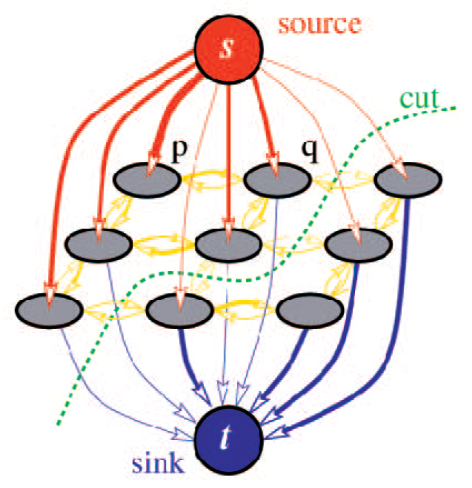
\includegraphics[width=0.3\textwidth]{mincut}%
      &
      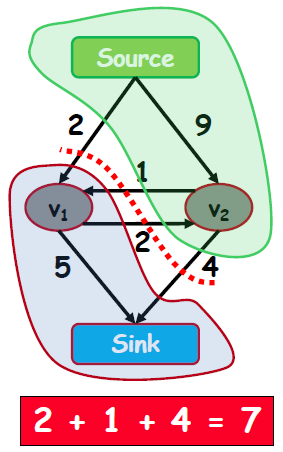
\includegraphics[width=0.2\textwidth]{min_cut}%
      &
      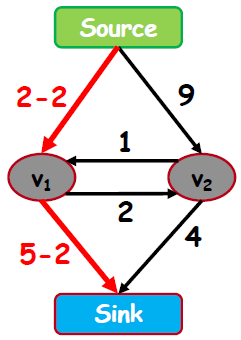
\includegraphics[width=0.2\textwidth]{max_flow}%
  \end{tabular}
\end{table}
\vfill














%%%%%%%%%%%%%%%%%%%%%%%%%%%%%%%%%%%%%%%%%%%%%%%%%%%%%%%%%%%%%%%%%%%%%%%%%%%%%%%%
\NewPage\headline{\LaTeX \ Tricks}
\vfill
Some \LaTeX\xspace tricks
\vfill




%%%%%%%%%%%%%%%%%%%%%%%%%%%%%%%%%%%%%%%%%%%%%%%%%%%%%%%%%%%%%%%%%%%%%%%%%%%%%%%%
\FinalPage
%%%

%%%


%%%%%%%%%%%%%%%%%%%%%%%%%%%%%%%%%%%%%%%%%%%%%%%%%%%%%%%%%%%%%%%%%%%%%%%%%%%%%%%%
\NewPage
%\headline{\refname}
%\renewcommand*{\refname}{}
\bibliographystyle{i6bibliostyle}
\bibliography{slides}

%\clearpage
\appendix
%%%%%%%%%%%%%%%%%%%%%%%%%%%%%%%%%%%%%%%%%%%%%%%%%%%%%%%%%%%%%%%%%%%%%%%%%%%%%%%%
\NewPage\headline{\appendixname: First Slide}
\vfill
\hypertarget{anchorname}{Hyper Target} on the first appendix slide. 
Look at the current page number.
\vfill



\end{document}
